% Gerado de CSVs agregados; dados numericos incorporados para portabilidade.
% Notebook SHA-256: e8ce396c21be212f5a12d673622adf543234983c3cd142088ea2dbe8e7621004
% Parecer SHA-256: 1ee24339005b98f24afb2375d080f1aaa8ff1ab0e8812427b8b103b890cef98a
% Requer: pgfplots, biblioteca statistics (somente taxas.tex).
% Ajuste opcional no chamador: \def\AlturaGrafico{4.4cm} e \def\LarguraGrafico{\linewidth}.
\begingroup
\providecommand{\AlturaGrafico}{4.4cm}
\providecommand{\LarguraGrafico}{\linewidth}
\definecolor{grafverde}{HTML}{24574D}
\definecolor{grafazul}{HTML}{1769A5}
\definecolor{grafgrafite}{HTML}{253A40}
\definecolor{graflaranja}{HTML}{B97736}
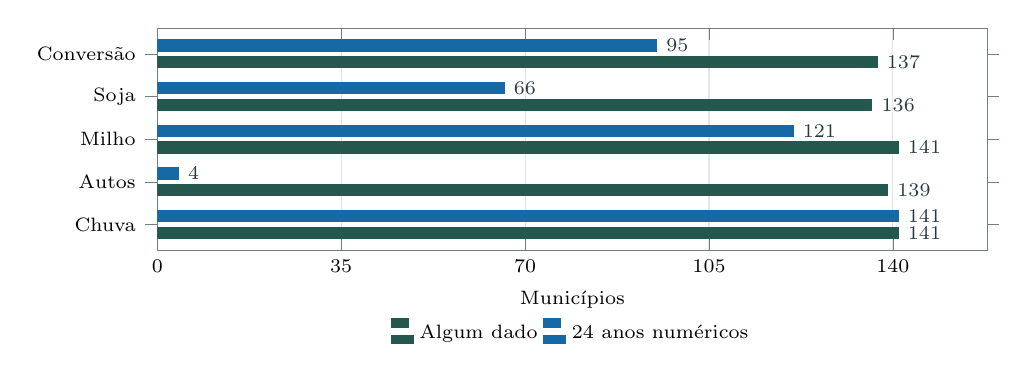
\begin{tikzpicture}
\begin{axis}[width=\LarguraGrafico,height=\AlturaGrafico,
font=\scriptsize,tick label style={font=\scriptsize},
label style={font=\scriptsize},
axis line style={grafgrafite!65},tick style={grafgrafite!65},
grid style={black!10},
legend style={font=\scriptsize,draw=none,fill=none,cells={anchor=west}},
/pgf/number format/use comma,
xbar,bar width=4pt,xmin=0,xmax=158,
xtick={0,35,70,105,140},ytick={1,2,3,4,5},
yticklabels={Convers\~ao,Soja,Milho,Autos,Chuva},
y dir=reverse,ymin=0.4,ymax=5.6,xmajorgrids=true,
xlabel={Munic\'ipios},
legend columns=2,legend style={at={(0.5,-0.28)},anchor=north},
nodes near coords={\pgfmathprintnumber[fixed,precision=0]{\pgfplotspointmeta}},
nodes near coords align={horizontal},
every node near coord/.append style={font=\scriptsize,text=grafgrafite},
]
\addplot+[draw=grafverde,fill=grafverde] coordinates {(137,1) (136,2) (141,3) (139,4) (141,5)};
\addplot+[draw=grafazul,fill=grafazul] coordinates {(95,1) (66,2) (121,3) (4,4) (141,5)};
\legend{Algum dado,24 anos num\'ericos}
\end{axis}
\end{tikzpicture}
\endgroup
